\section{\texorpdfstring{Dvojice množin}{Dvojice množin}}
\vspace{5mm}
\large

\begin{note}
	Motivace z logiky: pokud máme rozumnou teorii, tak určuje sentence které dokazuje a sentence které vyvrací.
	Když teorie je bezesporná, tak množiny jsou disjunktní.
\end{note}

\begin{definition}[Rekurzivní neoddělitelnost]
	Disjunktní dvojice množin $A, B$ jsou \emph{rekurzivně neoddělitelné} když neexistuje $M$ t.ž.
	\[ A \subseteq M \land M \cap B = \emptyset (B \subseteq \overline{M}) \]
\end{definition}

\begin{definition}[Efektivní neoddělitelnost]
	Disjunktní dvojice množin $A, B$ jsou \emph{efektivně neoddělitelné} když existuje $f \in ČRF$ t.ž.
	\[ \forall x, y: A \subseteq W_x \land B \subseteq W_y \land W_x \cap W_y = \emptyset \Rightarrow f(x, y) \downarrow \notin W_x \cup W_y \]
	Efektivně můžeme nejít bod který leží mimo obaly A, B.
\end{definition}

\begin{note}
	Efektivní neoddělitelnost $\Rightarrow$ rekurzivní neoddělitelnost.
\end{note}

\begin{theorem}[Efektivní neoddělitelné (BD)]
	Existuji rekurzivně neoddělitelné které nejsou efektivně neoddělitelné.
\end{theorem}
\begin{proof}
	Podobná konstrukce jako u Simple.
\end{proof}

\begin{note}
	Efektivní neoddělitelnost vždy lze definovat tak, aby $f \in ORF$ (neboli všude definovaná).
\end{note}

\begin{theorem}[Existence efektivní neoddělitelné]
	Existuji disjunktní r.s $E, F$ které jsou efektivně neoddělitelné.
\end{theorem}
\begin{proof}
	Znovu diagonální metoda.

	Vezmeme
	\[ E = \{ x|\ \varphi_x(x) \simeq 0 \} \]
	\[ F = \{ x|\ \varphi_x(x) \simeq 1 \} \]
	Na konkretních hodnotách nezáleží, šlo by vzít $i, j \in \N: i \ne j$.

	Hned je vidět, že $E, F$ jsou disjunktní a r.s.

	Podle s-m-n \cref{s_m_n} věty existuje PRF taková, že:
	\[ \varphi_{\alpha(x, y)} (w) =
		\left\{
		\begin{array}{lll}
			1 & \mbox{ } w \ \text{padne dříve do} \ W_x \ \text{než do} \ W_y \\
			0 & \mbox{ } w \ \text{padne dříve do} \ W_y \ \text{než do} \ W_x \\
			\uparrow & \mbox{ } w \notin W_x \cup W_x
		\end{array}
		\right.
	\]

	Formálně (dříve než ...)
	\[ \exists j (T_1(x, w, j) \land \forall i \leq j: \neg T_1(y, w, i)) \]

	Pokud oba dva programy skonči za stejný počet kroků, tak vezmeme libovolný.

	Nechť $W_x \supseteq E$ je rekurzivní obal $E$, nápodobně $W_y \supseteq F$.

	Uvažme
	\[ \varphi_{\alpha(x, y)}(\alpha(x, y)) \]
	Kdyby $\alpha(x, y)$ padlo do $W_x$, potom zřejmě padne dříve do $W_x$ než do $W_y$.
	Pak
	\[ \varphi_{\alpha(x, y)}(\alpha(x, y)) = 1 \]
	a tedy by muselo $\alpha(x, y)$ padnout do $F$. To nelze.

	Symetricky $\alpha(x, y)$ nemůže padnout do $W_y$ neboli
	\[ \alpha(x, y) \notin W_x \cup W_y \]

\end{proof}

\begin{note}
	Paradox lháře: tento výrok je lživý.
	Používá self-referenci.

	Ten ale operuje s pojmem pravdy, který není matematický.
	Můžeme ale podobný trik provést s např pojmem dokazatelnosti (viz Godelová 1. věta o neúplnosti \cref{godel}).
\end{note}

\begin{definition}[1-převoditelnost dvojic]
	Disjunktní dvojice
	\[ (C, D) \leq_1 (A, B) \]
	právě když existuje prostá $f \in ČRF$:
	\begin{gather*}
		x \in C \iff f(x) \in A\\
		x \in D \iff f(x) \in B\\
		x \notin C \cup D \iff f(x) \notin A \cup B
	\end{gather*}
\end{definition}

\begin{definition}[1-úplnost dvojic]
	Disjunktní dvojice r.s. množin $(A, B)$ je 1-úplná pravě když libovolná disjunktní dvojice r.s. množin $(C, D)$ platí:
	\[ (C, D) \leq_1 (A, B) \]
\end{definition}

\begin{theorem}[Dvojná věta o rekurzi]\label{rek_2x}
	Pro libovolné $f, g \in ORF$:
	\[ \exists m, n: \varphi_m = \varphi_{f(m, n)},\ \varphi_n = \varphi_{g(m, n)} \]

	Obecněji: pro libovolné $f, g \in ORF$, obě $(k + 2)$ proměnných, existují $w_1, w_2 \in PRF$:
	\[ \varphi_{w_1(y_1, \ldots, y_k)} = \varphi_{f(w_1(y_1, \ldots, y_k), w_2(y_1, \ldots, y_k), y_1, \ldots, y_k)} \]
	\[ \varphi_{w_2(y_1, \ldots, y_k)} = \varphi_{g(w_1(y_1, \ldots, y_k), w_2(y_1, \ldots, y_k), y_1, \ldots, y_k)} \]
\end{theorem}
\begin{proof}
	Z Věty o rekurzi \cref{rek_1} existuje $h \in ORF$:
	\[ \varphi_{h(y)} = \varphi_{f(h(y), y)} \]
	Vezmeme
	\[ \varphi_{g(h(y), y)}, \exists n: \varphi_n = \varphi_{g(h(n), n)} \]
	Položme $m = h(n)$.
\end{proof}

\begin{theorem}[Efektivní neoddělitelné, 1-úplnost]
	Disjunktní r.s dvojice množin jsou efektivně neoddělitelné $\iff$ jsou 1-úplné.
\end{theorem}
\begin{proof}
	"1-úplnost $\Rightarrow$ efektivní neoddělitelnost".

	Nechť $(C, D)$ efektivně neoddělitelné s funkci $f$ a $(C, D) \leq_1 (A, B)$ s funkci $g$, neboli $(C, D)$ je 1-úplná.

	Vezmeme vzory r.s. obalů $A \subseteq W_x, B \subseteq W_y$:
	\[ W_{\alpha(x)} = g^{-1}(W_x), W_{\alpha(y)} = g^{-1}(W_y) \]
	Jelikož, $(C, D)$ efektivně neoddělitelné $\Rightarrow W_{\alpha(x)} \cap W_{\alpha(y)} = \emptyset$.
	Taky funkce $f$ dá bod
	\[ new = f(\alpha(x), \alpha(y)): new \notin W_{\alpha(x)} \cup W_{\alpha(y)} \]
	Zobrazíme $new$ pomoci $g$ zpátky. Pak
	\[ g(new) = f \circ g(\alpha(x), \alpha(y)) \notin W_x \cup W_y\]
	Z čehož, $(A, B)$ je efektivně neoddělitelná.

	% obrazek, 5. lekce 53:29
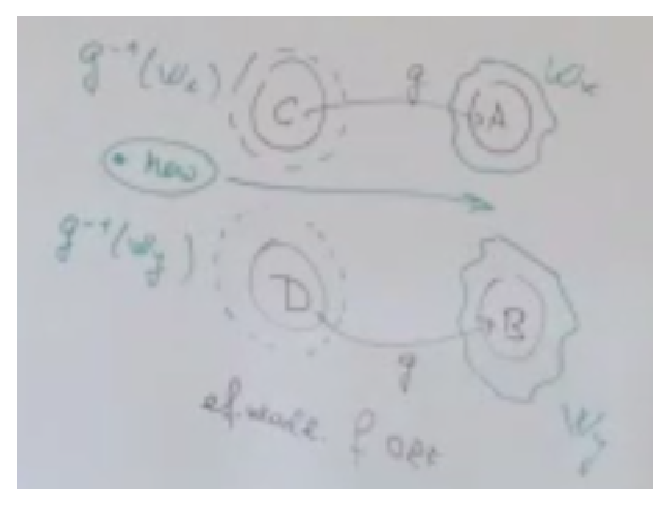
\includegraphics[scale=0.4]{2dis_0.eps}

	"1-úplnost $\Leftarrow$ efektivní neoddělitelnost".

	Nechť $(A, B)$ efektivně neoddělitelné s funkci $f \in ČRF$.
	Nechť $(C, D)$ libovolné disjunktní množiny.

	Sestavíme množiny
	\[ W_{w_1(x)} = \twopartdef { A \cup \{ f(w_1(x), w_2(x)) \} } { x \in D } { A } { x \notin D } \]
	\[ W_{w_2(x)} = \twopartdef { B \cup \{ f(w_1(x), w_2(x)) \} } { x \in C } { B } { x \notin C } \]
	Které dostaneme pomoci dvojné věty o rekurzi \cref{rek_2x}
	\[ W_{\alpha(y_1, y_2, x)} = \twopartdef { A \cup \{ f(y_1(x), y_2(x)) \} } { x \in D } { A } { x \notin D } \]
	\[ W_{\beta(y_1, y_2, x)} = \twopartdef { B \cup \{ f(y_1(x), y_2(x)) \} } { x \in C } { B } { x \notin C } \]


	Zkontrolujeme 2 případy:
	\[ x \notin C \cup D \Rightarrow W_{w_1(x)} = A, W_{w_2(x)} = B \Rightarrow f(w_1(x), w_2(x)) \notin A \cup B \]
	jinak např $x \in C \Rightarrow x \notin D$ protože jsou disjunktní dle předpokladu.
	Pak
	\[ W_{w_1(x)} = A, W_{w_2(x)} = B \cup \{ f(w_1(x), w_2(x)) \} \]
	Pokud $f(w_1(x), w_2(x)) \notin A$ tak množiny $W_{w_1(x)}, W_{w_2(x)}$ jsou obaly $A, B$.
	Pak z efektivní neoddělitelnosti $f$ by měla vracet nový bod, ležící mimo:
	\[ f(w_1(x), w_2(x)) \notin W_{w_1(x)} \cup W_{w_2(x)} \]
	což je spor s konstrukci $W_{w_2(x)}$, protože $f(w_1(x), w_2(x)) \in W_{w_2(x)}$.

	Symetricky pro $D$.

	Dohromady $f(w_1(x), w_2(x))$ 1-převádí $(C, D)$ k $(A, B)$.
\end{proof}
